\documentclass[aspectratio=169, 10pt]{beamer}

% Packages
\usepackage{graphicx}
\usepackage{booktabs}
\usepackage{listings}
\usepackage{xcolor}
\usepackage{amsmath}
\usepackage{amssymb}
\usepackage{tikz}
\usepackage{url}

% Theme Setup (CMU Style Approximation)
\usetheme{Madrid}
\usecolortheme{beaver} % Uses red/grey which is close to CMU colors
\definecolor{cmured}{RGB}{196, 18, 48}
\setbeamercolor{structure}{fg=cmured}
\setbeamercolor{title}{bg=cmured, fg=white}
\setbeamercolor{frametitle}{bg=black, fg=white}

% Code Listing Setup
\lstset{
    basicstyle=\ttfamily\small,
    keywordstyle=\color{blue}\bfseries,
    commentstyle=\color{gray},
    stringstyle=\color{green!50!black},
    breaklines=true,
    frame=single,
    language=SQL
}

% Title Info
\title{Relational Model \& Algebra}
\subtitle{15-445/645 Database Systems}
\author{Prof. Andy Pavlo}
\institute{Carnegie Mellon University}
\date{Fall 2024}

\begin{document}
%
% --- PAGE 1 ---
\begin{frame}
    \titlepage
    \centering
    
\includegraphics[width=0.3\textwidth]{extracted_p1_1_image.jpeg}
\end{frame}

% --- PAGE 2 ---
\begin{frame}
    \centering
    %\includegraphics[width=0.8\textwidth]{extracted_p2_1_} 
\end{frame}

% --- PAGE 3 ---
\begin{frame}{Reddit Context}
    \begin{columns}
        \column{0.5\textwidth}
        
\includegraphics[width=\textwidth]{extracted_p3_1_image.jpeg}
        \column{0.5\textwidth}
        \textit{"is 15-440 or 15-445 harder? ... I don't really have preference for content and would like to spend more of my time on other stuff..."}
    \end{columns}
\end{frame}

% --- PAGE 4 ---
\begin{frame}{Reddit Context}
    \centering
    
\includegraphics[width=0.8\textwidth]{extracted_p4_1_image.jpeg}
    \vspace{1em}
    \begin{quote}
        "Since you've already admitted that you don't want to pursue a database-centric lifestyle, then you should probably not take my course." - apavlo
    \end{quote}
\end{frame}

% --- PAGE 5 ---
\begin{frame}{Course Logistics}
    \begin{itemize}
        \item \textbf{Course Policies + Schedule:} Course Web Page
        \item \textbf{Discussion + Announcements:} Piazza
        \item \textbf{Homeworks + Projects:} Gradescope
        \item \textbf{Final Grades:} Canvas
        \item \textbf{Waitlist:} Six open seats (as of 12pm today)
    \end{itemize}
    \vspace{1em}
    \begin{itemize}
        \item Non-CMU students can complete all assignments using Gradescope (Code: WWWJZ5).
        \item \textbf{Do not post your solutions on Github.}
        \item \textbf{Do not email instructors / TAs for help.}
        \item Discord Channel: \url{https://discord.gg/YF7dMCg}
    \end{itemize}
\end{frame}

% --- PAGE 6 ---
\begin{frame}{Today's Agenda}
    \begin{enumerate}
        \item Database Systems Background
        \item Relational Model
        \item Relational Algebra
        \item Alternative Data Models
        \item Q\&A Session
    \end{enumerate}
\end{frame}

% --- PAGE 7 ---
\begin{frame}
    \centering
    \Huge \textbf{Databases}
\end{frame}

% --- PAGE 8 ---
\begin{frame}{Database}
    \Large
    \begin{itemize}
        \item Organized collection of inter-related data that models some aspect of the real-world.
        \item Databases are the core component of most computer applications.
    \end{itemize}
\end{frame}

% --- PAGE 9 ---
\begin{frame}{Database Example}
    \textbf{Goal:} Create a database that models a digital music store to keep track of artists and albums.
    \vspace{1em}
    \begin{itemize}
        \item Information we need to keep track of in our store:
        \begin{itemize}
            \item Information about Artists
            \item The Albums those Artists released
        \end{itemize}
    \end{itemize}
\end{frame}

% --- PAGE 10 ---
\begin{frame}[fragile]{Flat File Strawman}
    \textbf{Proposal:} Store our database as comma-separated value (CSV) files that we manage ourselves in application code.
    \begin{itemize}
        \item Use a separate file per entity.
        \item The application must parse the files each time they want to read/update records.
    \end{itemize}
    \vspace{0.5em}
    \begin{columns}
        \column{0.5\textwidth}
        \textbf{Artist(name, year, country)}
\begin{verbatim}
"Wu-Tang Clan", 1992, "USA"
"Notorious BIG", 1992, "USA"
"GZA", 1990, "USA"
\end{verbatim}
        \column{0.5\textwidth}
        \textbf{Album(name, artist, year)}
\begin{verbatim}
"Enter the Wu-Tang", "Wu-Tang Clan", 1993
"St.Ides Mix Tape", "Wu-Tang Clan", 1994
"Liquid Swords", "GZA", 1990
\end{verbatim}
    \end{columns}
\end{frame}

% --- PAGE 11 ---
\begin{frame}[fragile]{Flat File Strawman}
    \textbf{Example:} Get the year that GZA went solo.
\begin{lstlisting}[language=Python]
for line in file.readlines():
    record = parse(line)
    if record[0] == "GZA":
        print(int(record[1]))
\end{lstlisting}

    \vspace{1em}
    \textbf{Input File:}
\begin{verbatim}
"Wu-Tang Clan",1992,"USA"
"Notorious BIG",1992,"USA"
"GZA",1990,"USA"
\end{verbatim}
\end{frame}

% --- PAGE 12 ---
\begin{frame}{Flat Files: Data Integrity}
    \begin{itemize}
        \item How do we ensure that the artist is the same for each album entry?
        \item What if somebody overwrites the album year with an invalid string?
        \item What if there are multiple artists on an album?
        \item What happens if we delete an artist that has albums?
    \end{itemize}
\end{frame}

% --- PAGE 13 ---
\begin{frame}{Flat Files: Implementation}
    \begin{itemize}
        \item How do you find a particular record?
        \item What if we now want to create a new application that uses the same database?
        \item What if that application is running on a different machine?
        \item What if two threads try to write to the same file at the same time?
    \end{itemize}
\end{frame}

% --- PAGE 14 ---
\begin{frame}{Flat Files: Durability}
    \begin{itemize}
        \item What if the machine crashes while our program is updating a record?
        \item What if we want to replicate the database on multiple machines for high availability?
    \end{itemize}
\end{frame}

% --- PAGE 15 ---
\begin{frame}{Database Management System}
    \textbf{Definition:} A database management system (DBMS) is software that allows applications to store and analyze information in a database.
    \vspace{1em}
    \begin{itemize}
        \item A general-purpose DBMS supports the definition, creation, querying, update, and administration of databases in accordance with some data model.
    \end{itemize}
\end{frame}

% --- PAGE 16 ---
\begin{frame}{Data Models}
    \textbf{Data Model:} A collection of concepts for describing the data in a database.
    \vspace{1em}
    \textbf{Schema:} A description of a particular collection of data, using a given data model.
    \begin{itemize}
        \item $\rightarrow$ This defines the structure of data for a data model.
        \item $\rightarrow$ Otherwise, you have random bits with no meaning.
    \end{itemize}
\end{frame}

% --- PAGE 18 ---
\begin{frame}{Data Models}
    \begin{columns}
        \column{0.5\textwidth}
        \begin{itemize}
            \item \textbf{Relational} $\leftarrow$ Most DBMSs
            \item Key/Value
            \item Graph
            \item Document / JSON / XML / Object
            \item Wide-Column / Column-family
            \item Array (Vector, Matrix, Tensor)
            \item Hierarchical
            \item Network
        \end{itemize}
        \column{0.5\textwidth}
    \end{columns}
\end{frame}

% --- PAGE 19 ---
\begin{frame}{Data Models}
    \begin{columns}
        \column{0.5\textwidth}
        \begin{itemize}
            \item Relational
            \item \textbf{Key/Value} $\leftarrow$ Simple Apps / Caching
            \item Graph
            \item Document / JSON / XML / Object
            \item Wide-Column / Column-family
            \item Array (Vector, Matrix, Tensor)
            \item Hierarchical
            \item Network
        \end{itemize}
    \end{columns}
\end{frame}

% --- PAGE 20 ---
\begin{frame}{Data Models}
    \begin{columns}
        \column{0.5\textwidth}
        \begin{itemize}
            \item Relational
            \item Key/Value
            \item \textbf{Graph}
            \item \textbf{Document / JSON / XML / Object} $\leftarrow$ NoSQL
            \item \textbf{Wide-Column / Column-family}
            \item Array (Vector, Matrix, Tensor)
            \item Hierarchical
            \item Network
        \end{itemize}
    \end{columns}
\end{frame}

% --- PAGE 21 ---
\begin{frame}{Data Models}
    \begin{columns}
        \column{0.5\textwidth}
        \begin{itemize}
            \item Relational
            \item Key/Value
            \item Graph
            \item Document / JSON / XML / Object
            \item Wide-Column / Column-family
            \item \textbf{Array (Vector, Matrix, Tensor)} $\leftarrow$ ML / Science
            \item Hierarchical
            \item Network
        \end{itemize}
    \end{columns}
\end{frame}

% --- PAGE 22 ---
\begin{frame}{Data Models}
    \begin{columns}
        \column{0.5\textwidth}
        \begin{itemize}
            \item Relational
            \item Key/Value
            \item Graph
            \item Document / JSON / XML / Object
            \item Wide-Column / Column-family
            \item Array (Vector, Matrix, Tensor)
            \item \textbf{Hierarchical} $\leftarrow$ Obsolete / Legacy / Rare
            \item \textbf{Network}
        \end{itemize}
    \end{columns}
\end{frame}

% --- PAGE 23 ---
\begin{frame}{Data Models}
    \begin{columns}
        \column{0.5\textwidth}
        \begin{itemize}
            \item \textbf{Relational} $\leftarrow$ This Course
            \item Key/Value
            \item Graph
            \item Document / JSON / XML / Object
            \item Wide-Column / Column-family
            \item Array (Vector, Matrix, Tensor)
            \item Hierarchical
            \item Network
        \end{itemize}
    \end{columns}
\end{frame}

% --- PAGE 24 ---
\begin{frame}{Early DBMSs}
    Early database applications were difficult to build and maintain on available DBMSs in the 1960s.
    \begin{itemize}
        \item $\rightarrow$ Examples: IDS, IMS, CODASYL
        \item $\rightarrow$ Computers were expensive, humans were cheap.
    \end{itemize}
    \vspace{1em}
    Tight coupling between logical and physical layers.
    \begin{itemize}
        \item Programmers had to (roughly) know what queries the application would execute before they could deploy the database.
    \end{itemize}
\end{frame}

% --- PAGE 25 ---
\begin{frame}{Early DBMSs}
    \begin{columns}
        \column{0.6\textwidth}
        \textbf{Edgar F. Codd}
        \begin{itemize}
            \item Ted Codd was a mathematician at IBM Research in the late 1960s.
            \item Codd saw IBM’s developers rewriting database programs every time the database’s schema or layout changed.
            \item Devised the relational model in 1969.
        \end{itemize}
        \column{0.4\textwidth}
        \centering
        
\includegraphics[width=0.8\textwidth]{extracted_p25_1_image.png}
    \end{columns}
\end{frame}

% --- PAGE 26 ---
\begin{frame}{Relational Model (1970)}
    \centering
    
\includegraphics[width=0.3\textwidth]{extracted_p26_1_image.png} \hspace{0.5em}
    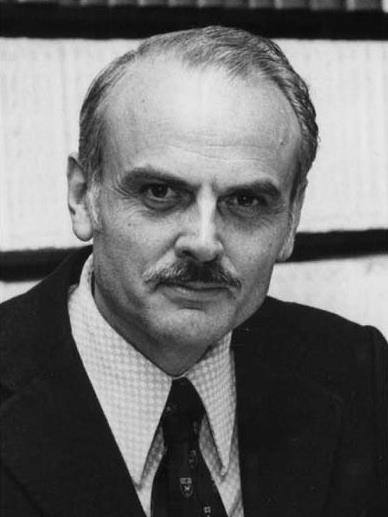
\includegraphics[width=0.3\textwidth]{extracted_p26_2_image.jpeg} \hspace{0.5em}
    
\includegraphics[width=0.3\textwidth]{extracted_p26_3_image.png}
    \\
    \textit{"A Relational Model of Data for Large Shared Data Banks" - CACM 1970}
\end{frame}

% --- PAGE 27 ---
\begin{frame}{CODASYL}
    \begin{itemize}
        \item ACM SIGFIDET Workshop on Data Description, Access, and Control in Ann Arbor, Michigan, held 1–3 May 1974
        \item The Differences and Similarities Between the Data Base Set and Relational Views of Data.
    \end{itemize}
    \centering
    
\includegraphics[width=0.8\textwidth]{extracted_p27_1_image.png}
\end{frame}

% --- PAGE 28 ---
\begin{frame}{The Great Debate (1974)}
    \begin{columns}
        \column{0.5\textwidth}
        \textbf{COBOL/CODASYL camp (Bachman):}
        \begin{enumerate}
            \item The relational model is too mathematical. No mere mortal programmer will understand it.
            \item You won't be able to build an efficient implementation.
            \item OLTP apps want record-oriented operations.
        \end{enumerate}
        \column{0.5\textwidth}
        \textbf{Relational camp (Codd/Stonebraker):}
        \begin{enumerate}
            \item Nothing as complicated as CODASYL can be the right way.
            \item Set-oriented queries are too hard in CODASYL DML.
            \item CODASYL model has no formal underpinning.
        \enumerate}
    \end{columns}
    \vspace{1em}
    \centering
    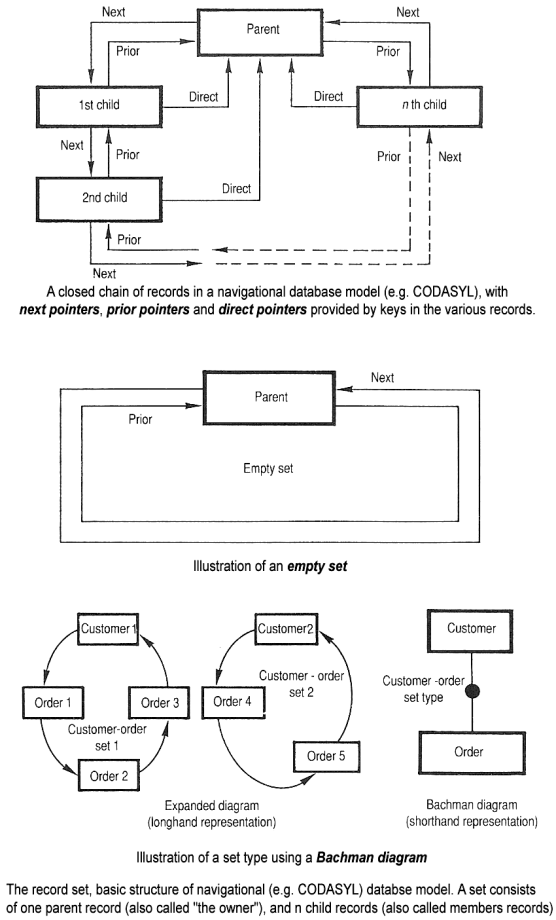
\includegraphics[height=1.5cm]{extracted_p27_2_image.png}
    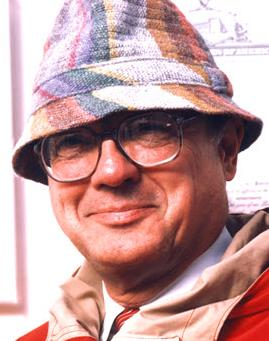
\includegraphics[height=1.5cm]{extracted_p27_3_image.jpeg}
    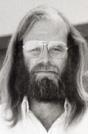
\includegraphics[height=1.5cm]{extracted_p27_4_image.jpeg}
    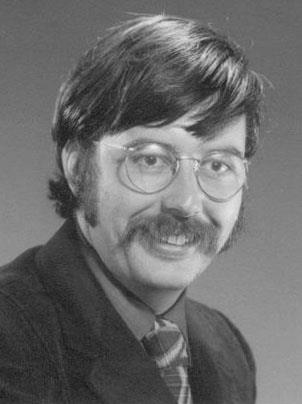
\includegraphics[height=1.5cm]{extracted_p27_5_image.jpeg}
\end{frame}

% --- PAGE 29 ---
\begin{frame}{Relational Model}
    The relational model defines a database abstraction based on relations to avoid maintenance overhead.
    \vspace{1em}
    \textbf{Key tenets:}
    \begin{itemize}
        \item Store database in simple data structures (relations).
        \item Physical storage left up to the DBMS implementation.
        \item Access data through high-level language; DBMS figures out best execution strategy.
    \end{itemize}
\end{frame}

% --- PAGE 30 ---
\begin{frame}{Relational Model}
    \begin{itemize}
        \item Relations have attributes (columns) and tuples (rows).
        \item Each attribute has a domain of allowed values.
        \item All tuples in a relation have the same attributes.
    \end{itemize}
\end{frame}
%
% --- PAGE 31 ---
\begin{frame}{Data Independence}
    Isolate the user/application from low level data representation.
    \begin{columns}
        \column{0.6\textwidth}
        \begin{itemize}
            \item $\rightarrow$ The user only worries about high-level application logic.
            \item $\rightarrow$ DBMS optimizes the layout according to operating environment, database contents, and workload.
            \item $\rightarrow$ DBMS can then re-optimize the database if/when these factors change.
        \end{itemize}
        \column{0.4\textwidth}
        
\includegraphics[width=\textwidth]{extracted_p31_1_image.png}
    \end{columns}
\end{frame}

% --- PAGE 32 ---
\begin{frame}{Relational Model Structure}
    \begin{itemize}
        \item A \textbf{relation} is an unordered set that contains the relationship of attributes that represent entities.
        \item A \textbf{tuple} is a set of attribute values in the relation.
        \begin{itemize}
            \item Values are (normally) atomic/scalar.
            \item The value NULL is a member of every domain (if allowed).
        \end{itemize}
    \end{itemize}

    \vspace{1em}
    \textbf{n-ary Relation = Table with n columns}

    \small
    \begin{table}
    \begin{tabular}{lll}
    \toprule
    \textbf{name} & \textbf{year} & \textbf{country} \\
    \midrule
    Wu-Tang Clan & 1992 & USA \\
    Notorious BIG & 1992 & USA \\
    GZA & 1990 & USA \\
    \bottomrule
    \end{tabular}
    \caption{Artist(name, year, country)}
    \end{table}
\end{frame}

% --- PAGE 33 ---
\begin{frame}{Relational Model: Primary Keys}
    \begin{columns}
        \column{0.6\textwidth}
        \begin{itemize}
            \item A relation's \textbf{primary key} uniquely identifies a single tuple.
            \item Some DBMSs automatically create an internal primary key if a table does not define one.
            \item DBMS can auto-generate primary keys:
            \begin{itemize}
                \item \texttt{IDENTITY}
                \item \texttt{SEQUENCE}
                \item \texttt{AUTO\_INCREMENT}
            \end{itemize}
        \end{itemize}

        \column{0.4\textwidth}
        \small
        \textbf{Artist(name, year, country)}
        \begin{table}
        \begin{tabular}{lll}
        \toprule
        name & year & country \\
        \midrule
        Wu-Tang Clan & 1992 & USA \\
        Notorious BIG & 1992 & USA \\
        GZA & 1990 & USA \\
        \bottomrule
        \end{tabular}
        \end{table}
    \end{columns}
\end{frame}

% --- PAGE 34 ---
\begin{frame}{Relational Model: Primary Keys}
    \begin{columns}
        \column{0.6\textwidth}
        \textbf{Example with ID column:}

        \column{0.4\textwidth}
        \small
        \textbf{Artist(id, name, year, country)}
        \begin{table}
        \begin{tabular}{llll}
        \toprule
        id & name & year & country \\
        \midrule
        101 & Wu-Tang Clan & 1992 & USA \\
        102 & Notorious BIG & 1992 & USA \\
        103 & GZA & 1990 & USA \\
        \bottomrule
        \end{tabular}
        \end{table}
    \end{columns}
\end{frame}

% --- PAGE 35 ---
\begin{frame}{Relational Model: Foreign Keys}
    \textbf{A foreign key} specifies that an attribute in one relation maps to a tuple in another relation.
\end{frame}

% --- PAGE 36 ---
\begin{frame}{Relational Model: Foreign Keys}
    \begin{columns}
        \column{0.5\textwidth}
        \textbf{Album(id, name, artist, year)}
        \begin{table}
        \tiny
        \begin{tabular}{llll}
        \toprule
        id & name & artist & year \\
        \midrule
        11 & Enter the Wu-Tang & 101 & 1993 \\
        22 & St. Ides Mix Tape & ??? & 1994 \\
        33 & Liquid Swords & 103 & 1995 \\
        \bottomrule
        \end{tabular}
        \end{table}

        \column{0.5\textwidth}
        \textbf{Artist(id, name, year, country)}
        \begin{table}
        \tiny
        \begin{tabular}{llll}
        \toprule
        id & name & year & country \\
        \midrule
        101 & Wu-Tang Clan & 1992 & USA \\
        102 & Notorious BIG & 1992 & USA \\
        103 & GZA & 1990 & USA \\
        \bottomrule
        \end{tabular}
        \end{table}
    \end{columns}
\end{frame}

% --- PAGE 37 ---
\begin{frame}{Relational Model: Foreign Keys}
    \textbf{Mapping Table for Many-to-Many}

    \begin{center}
        \textbf{ArtistAlbum(artist\_id, album\_id)}
        \begin{table}
        \begin{tabular}{ll}
        \toprule
        artist\_id & album\_id \\
        \midrule
        101 & 11 \\
        101 & 22 \\
        103 & 22 \\
        102 & 22 \\
        \bottomrule
        \end{tabular}
        \end{table}
    \end{center}
\end{frame}

% --- PAGE 38 ---
\begin{frame}{Relational Model: Foreign Keys}
    \centering
    
\includegraphics[width=0.8\textwidth]{extracted_p38_1_image.png}
\end{frame}

% --- PAGE 39 ---
\begin{frame}[fragile]{Relational Model: Constraints}
    \begin{columns}
        \column{0.6\textwidth}
        \begin{itemize}
            \item User-defined conditions that must hold for all tuples.
            \item Can check values in one tuple or across tuples.
            \item DBMS blocks modifications that violate constraints.
        \end{itemize}

        \column{0.4\textwidth}
        \begin{lstlisting}[language=SQL]
CREATE TABLE Artist (
    name VARCHAR NOT NULL,
    year INT,
    country CHAR(60),
    CHECK (year > 1900)
);
        \end{lstlisting}
    \end{columns}
\end{frame}

% --- PAGE 40 ---
\begin{frame}{Data Manipulation Languages (DML)}
    API for storing and retrieving data.
    \vspace{1em}

    \begin{itemize}
        \item \textbf{Procedural} (Relational Algebra): describe how to get data.
        \item \textbf{Declarative} (Relational Calculus): describe what data you want.
    \end{itemize}
\end{frame}

% --- PAGE 41 ---
\begin{frame}{Relational Algebra}
    \begin{itemize}
        \item Based on set algebra.
        \item Operators take relations as input and produce new relations.
    \end{itemize}

    \vspace{1em}
    \begin{columns}
        \column{0.5\textwidth}
        \begin{itemize}
            \item $\sigma$ Select
            \item $\pi$ Projection
            \item $\cup$ Union
            \item $\cap$ Intersection
        \end{itemize}

        \column{0.5\textwidth}
        \begin{itemize}
            \item $-$ Difference
            \item $\times$ Product
            \item $\bowtie$ Join
        \end{itemize}
    \end{columns}
\end{frame}

% --- PAGE 42 ---
\begin{frame}{Relational Algebra: Select}
    Select tuples in a relation that satisfy a predicate.
    \begin{itemize}
        \item Predicate acts as a filter.
        \item Can combine predicates with AND, OR.
    \end{itemize}

    \vspace{1em}
    \textbf{Syntax:} $\sigma_{predicate}(R)$

    \vspace{1em}
    Example: $\sigma_{a\_id='a2' \land b\_id>102}(R)$
\end{frame}

\end{document}

\begin{frame}[fragile]{Relational Algebra: Select}
\begin{columns}

% ----- COLUMN 1 -----
\column{0.3\textwidth}
\textbf{R(a\_id, b\_id)}

\tiny
\begin{tabular}{ll}
\toprule
a\_id & b\_id \\
\midrule
a1 & 101 \\
a2 & 102 \\
a2 & 103 \\
a3 & 104 \\
\bottomrule
\end{tabular}

% ----- COLUMN 2 -----
\column{0.3\textwidth}
$\sigma_{a\_id = \text{'a2'}}(R)$

\tiny
\begin{tabular}{ll}
\toprule
a\_id & b\_id \\
\midrule
a2 & 102 \\
a2 & 103 \\
\bottomrule
\end{tabular}

% ----- COLUMN 3 -----
\column{0.4\textwidth}
\begin{lstlisting}[language=SQL]
SELECT * FROM R
WHERE a_id='a2' 
  AND b_id>102;
\end{lstlisting}

\end{columns}
\end{frame}



% --- PAGE 44 ---
\begin{frame}[fragile]{Relational Algebra: Projection}
    Generate a relation with tuples that contains only the specified attributes.
    \begin{itemize}
        \item $\rightarrow$ Rearrange attributes’ ordering.
        \item $\rightarrow$ Remove unwanted attributes.
        \item $\rightarrow$ Manipulate values to create derived attributes.
    \end{itemize}
    \vspace{1em}
    \textbf{Syntax:} $\Pi_{A1,A2,\dots,An}(R)$
    \vspace{1em}
    \begin{columns}
        \column{0.5\textwidth}
        $\Pi_{b\_id-100,a\_id}(\sigma_{a\_id='a2'}(R))$
        \column{0.5\textwidth}
        \begin{lstlisting}[language=SQL]
SELECT b_id-100, a_id
FROM R WHERE a_id = 'a2';
        \end{lstlisting}
    \end{columns}
\end{frame}

% --- PAGE 45 ---
\begin{frame}[fragile]{Relational Algebra: Union}
    Generate a relation that contains all tuples that appear in either only one or both input relations.
    \vspace{1em}
    \textbf{Syntax:} $(R \cup S)$
    \vspace{1em}
    \begin{columns}
        \column{0.5\textwidth}
        \begin{itemize}
            \item Standard set algebra rules apply.
        \end{itemize}
        \column{0.5\textwidth}
        \begin{lstlisting}[language=SQL]
(SELECT * FROM R)
UNION
(SELECT * FROM S);
        \end{lstlisting}
    \end{columns}
\end{frame}

% --- PAGE 46 ---
\begin{frame}[fragile]{Relational Algebra: Intersection}
    Generate a relation that contains only the tuples that appear in both of the input relations.
    \vspace{1em}
    \textbf{Syntax:} $(R \cap S)$
    \vspace{1em}
    \begin{columns}
        \column{0.5\textwidth}
        \textbf{R} (a1, a2, a3) \\ \textbf{S} (a3, a4, a5) \\
        $\rightarrow$ Result: (a3)
        \column{0.5\textwidth}
        \begin{lstlisting}[language=SQL]
(SELECT * FROM R)
INTERSECT
(SELECT * FROM S);
        \end{lstlisting}
    \end{columns}
\end{frame}

% --- PAGE 47 ---
\begin{frame}[fragile]{Relational Algebra: Difference}
    Generate a relation that contains only the tuples that appear in the first and not the second of the input relations.
    \vspace{1em}
    \textbf{Syntax:} $(R - S)$
    \vspace{1em}
    \begin{columns}
        \column{0.5\textwidth}
        \textbf{R} (a1, a2, a3) \\ \textbf{S} (a3, a4, a5) \\
        $\rightarrow$ Result: (a1, a2)
        \column{0.5\textwidth}
        \begin{lstlisting}[language=SQL]
(SELECT * FROM R)
EXCEPT
(SELECT * FROM S);
        \end{lstlisting}
    \end{columns}
\end{frame}

% --- PAGE 48 ---
\begin{frame}[fragile]{Relational Algebra: Product}
    Generate a relation that contains all possible combinations of tuples from the input relations.
    \vspace{1em}
    \textbf{Syntax:} $(R \times S)$
    \vspace{1em}
    \begin{lstlisting}[language=SQL]
SELECT * FROM R CROSS JOIN S;
SELECT * FROM R, S;
    \end{lstlisting}
\end{frame}

% --- PAGE 49 ---
\begin{frame}{Relational Algebra: Join}
    Generate a relation that contains all tuples that are a combination of two tuples (one from each input relation) with a common value(s) for one or more attributes.
    \vspace{1em}
    \textbf{Syntax:} $(R \bowtie S)$
\end{frame}

% --- PAGE 50-52 (Join Animations) ---
\begin{frame}[fragile]{Relational Algebra: Join (Examples)}
    \begin{columns}
        \column{0.5\textwidth}
        \textbf{R(a\_id, b\_id)}
        \begin{table}\tiny \begin{tabular}{ll} a1 & 101 \\ a2 & 102 \\ a3 & 103 \end{tabular} \end{table}
        \textbf{S(a\_id, b\_id, val)}
        \begin{table}\tiny \begin{tabular}{lll} a3 & 103 & XXX \\ a4 & 104 & YYY \\ a5 & 105 & ZZZ \end{tabular} \end{table}
        
        \column{0.5\textwidth}
        \textbf{Result $(R \bowtie S)$:}
        \begin{table}\tiny \begin{tabular}{lll} a3 & 103 & XXX \end{tabular} \end{table}
        
        \begin{lstlisting}[language=SQL, basicstyle=\tiny\ttfamily]
SELECT * FROM R NATURAL JOIN S;
SELECT * FROM R JOIN S USING (a_id, b_id);
SELECT * FROM R JOIN S ON R.a_id = S.a_id;
        \end{lstlisting}
    \end{columns}
\end{frame}

% --- PAGE 53 ---
\begin{frame}{Relational Algebra: Extra Operators}
    \begin{itemize}
        \item Rename ($\rho$)
        \item Assignment ($R \leftarrow S$)
        \item Duplicate Elimination ($\delta$)
        \item Aggregation ($\gamma$)
        \item Sorting ($\tau$)
        \item Division ($R \div S$)
    \end{itemize}
\end{frame}

% --- PAGE 54 ---
\begin{frame}{Observation}
    Relational algebra defines an ordering of the high level steps of how to compute a query.
    \begin{itemize}
        \item $\rightarrow$ Example: $\sigma_{b\_id=102}(R \bowtie S)$ vs. $(R \bowtie (\sigma_{b\_id=102}(S)))$
    \end{itemize}
    \vspace{1em}
    A better approach is to state the high-level answer that you want the DBMS to compute.
    \begin{itemize}
        \item $\rightarrow$ Example: Retrieve the joined tuples from R and S where b\_id equals 102.
    \end{itemize}
\end{frame}

% --- PAGE 55 ---
\begin{frame}[fragile]{Relational Model: Queries}
    The relational model is independent of any query language implementation.
    \begin{itemize}
        \item SQL is the de facto standard (many dialects).
    \end{itemize}
    \vspace{1em}
    \begin{columns}
        \column{0.5\textwidth}
        \begin{lstlisting}[language=Python]
for line in file:
 record = parse(line)
 if record[0] == "GZA":
  print(int(record[1]))
        \end{lstlisting}
        \column{0.5\textwidth}
        \begin{lstlisting}[language=SQL]
SELECT year FROM artists
WHERE name = 'GZA';
        \end{lstlisting}
    \end{columns}
\end{frame}

% --- PAGE 56 ---
\begin{frame}{Data Models}
    \begin{itemize}
        \item \textbf{Relational} $\leftarrow$ This Course
        \item Key/Value
        \item Graph
        \item Document / JSON / XML / Object
        \item Wide-Column / Column-family
        \item Array (Vector, Matrix, Tensor)
    \end{itemize}
\end{frame}

% --- PAGE 57 ---
\begin{frame}{Data Models}
    \begin{itemize}
        \item Relational
        \item Key/Value
        \item Graph
        \item \textbf{Document / JSON / XML / Object} $\leftarrow$ Leading Alternative
        \item Wide-Column / Column-family
        \item \textbf{Array (Vector, Matrix, Tensor)} $\leftarrow$ New Hotness
    \end{itemize}
\end{frame}

% --- PAGE 58 ---
\begin{frame}{Document Data Model}
    A collection of record documents containing a hierarchy of named field/value pairs.
    \begin{itemize}
        \item $\rightarrow$ A field’s value can be either a scalar type, an array of values, or another document.
        \item $\rightarrow$ Modern implementations use JSON. Older systems use XML or custom object representations.
    \end{itemize}
    \vspace{1em}
    Avoid “relational-object impedance mismatch” by tightly coupling objects and database.
    \centering
    
\includegraphics[height=1.5cm]{extracted_p58_1_image.png} % MongoDB Logo
    
\includegraphics[height=1.5cm]{extracted_p58_2_image.png} % CouchDB Logo
\end{frame}

% --- PAGE 59 & 60 ---
\begin{frame}{Document Data Model (Relational Version)}
    \centering
    \textbf{Artist} $\bowtie$ \textbf{ArtistAlbum} $\bowtie$ \textbf{Album}
    \vspace{1em}
    \\
    $R1(id,\dots)$ \hspace{1em} $R2(artist\_id,album\_id)$ \hspace{1em} $R3(id,\dots)$
\end{frame}

% --- PAGE 61 & 62 ---
\begin{frame}[fragile]{Document Data Model (JSON vs Code)}
    \begin{columns}
        \column{0.5\textwidth}
        \textbf{Document / JSON}
        \begin{verbatim}
{
 "name": "GZA",
 "year": 1990,
 "albums": [
  {
   "name": "Liquid Swords",
   "year": 1995
  },
  ...
 ]
}
        \end{verbatim}
        \column{0.5\textwidth}
        \textbf{Application Code (Java/C++)}
        \begin{verbatim}
class Artist {
  int id;
  String name;
  int year;
  Album albums[];
}
        \end{verbatim}
    \end{columns}
\end{frame}

% --- PAGE 63 & 64 ---
\begin{frame}{Vector Data Model}
    One-dimensional arrays used for nearest-neighbor search (exact or approximate).
    \begin{itemize}
        \item $\rightarrow$ Used for semantic search on embeddings generated by ML trained transformer models (think ChatGPT).
        \item $\rightarrow$ Native integration with modern ML tools and APIs (e.g., LangChain, OpenAI).
    \end{itemize}
    At their core, these systems use specialized indexes to perform NN searches quickly.
    \vspace{1em}
    \centering
    
\includegraphics[height=1cm]{extracted_p63_1_image.png} % Pinecone
    
\includegraphics[height=1cm]{extracted_p63_2_image.png} % Weaviate
    
\includegraphics[height=1cm]{extracted_p63_3_image.png} % Qdrant
    
\includegraphics[height=1cm]{extracted_p63_4_image.png} % Milvus
\end{frame}

% --- PAGE 65 ---
\begin{frame}{Vector Data Model}
    \centering
    
\includegraphics[width=0.8\textwidth]{extracted_p65_1_image.png}
    % Diagram: Text -> Embeddings -> Vector Index (HNSW)
\end{frame}

% --- PAGE 66 ---
\begin{frame}{Vector Data Model}
    \centering
    
\includegraphics[width=0.8\textwidth]{extracted_p66_1_image.png}
    % Diagram: Query -> Transformer -> Vector -> Search
\end{frame}

% --- PAGE 67 ---
\begin{frame}{Vector Data Model}
    \centering
    
\includegraphics[width=0.8\textwidth]{extracted_p67_1_image.png}
    % Diagram: Full flow to Ranked List of Ids
\end{frame}

% --- PAGE 68 ---
\begin{frame}{Conclusion}
    \begin{itemize}
        \item Databases are ubiquitous.
        \item Relational algebra defines the primitives for processing queries on a relational database.
        \item We will see relational algebra again when we talk about query optimization + execution.
    \end{itemize}
\end{frame}

% --- PAGE 69 ---
\begin{frame}{Next Class}
    \Large
    \textbf{Modern SQL}
    \vspace{1em}
    \normalsize
    \begin{itemize}
        \item $\rightarrow$ Make sure you understand basic SQL before the lecture.
    \end{itemize}
\end{frame}

% --- PAGE 70 ---
\begin{frame}[fragile]{Ask Andy Anything}
    \begin{itemize}
        \item Questions about database industry?
        \item Questions about database jobs?
        \item Questions about database systems?
    \end{itemize}
\end{frame}

\end{document}